\documentclass[final,5p,times,twocolumn]{elsarticle}

% ---------- PACKAGES ----------
\usepackage{amsmath,amssymb,amsfonts,mathtools,bm}
\usepackage{amsthm}
%\usepackage[numbers,sort&compress]{natbib} % enabled for citations
\usepackage{hyperref}
\hypersetup{colorlinks=true,linkcolor=blue,citecolor=blue,urlcolor=blue}
\usepackage{tikz}
\usetikzlibrary{arrows.meta,calc,3d,bending, decorations.markings}

% ---------- THEOREM ENVIRONMENTS ----------
\newtheorem{theorem}{Theorem}
\newtheorem{proposition}{Proposition}
\newtheorem{lemma}{Lemma}
\newtheorem{assumption}{Assumption}
\newtheorem{definition}{Definition}
\newtheorem{remark}{Remark}

% ---------- SHORTCUTS ----------
\DeclareMathOperator{\tr}{tr}
\newcommand{\R}{\mathbb{R}}
\newcommand{\diff}{\mathrm{d}}

% ---------- TITLE ----------
\journal{Automatica}

\begin{document}
	
	\begin{frontmatter}
		
		% ----- TITLE SWITCHER (leave commented; uncomment exactly one if you wish) -----
		\title{Routing Information, Not Power: Skew Interconnections in Port--Hamiltonian Systems} % option 1
		% \title{The Information Geometry of Skew: Tuning Port--Hamiltonian Interconnections}       % option 2
		% \title{Geometric Information Control: Shaping Skew Interconnections in Port--Hamiltonian Systems} % option 3
		
		% \title{Skew Interconnections as Information Routers in Nonlinear Port--Hamiltonian Systems:\\
%			Belief--Entropy Split, Mutual Information \& Vector Transfer Entropy, and Estimator--Level Guarantees}
		
		\author[]{Jasper Juchem\corref{cor1}}
		\cortext[cor1]{Corresponding author.}
		\ead{<your.email@domain>}
		\address{<Your Department and Institution>}
		
		\begin{abstract}
			We develop a theory of \emph{information--aware} interconnection shaping for nonlinear port--Hamiltonian (pH) systems in canonical symplectic coordinates. The skew--symmetric interconnection \(J(x)\) is classically known to be power--preserving. Here we show that, in the presence of stochastic disturbances and partial sensing, \(J(x)\) can be \emph{tuned} to \emph{route information} across a state partition and thereby accelerate the collapse of estimator uncertainty under fixed dissipation and diffusion. The theory proceeds in three steps. First, we state and prove a \emph{belief--entropy} rate decomposition (Fokker--Planck/Liouville) for stochastic pH dynamics: the Hamiltonian (skew) flow is volume--preserving and thus entropy--neutral, whereas dissipative and diffusive terms set the net entropy production. Second, we formalize \emph{block mutual information} (MI) and \emph{vector} transfer entropy (TE) across a partition as operational design signals, computed on the innovations of a Kalman--type filter; in linear--Gaussian cases, vector TE reduces to a log--det likelihood--ratio statistic. Third, under mild differential/dominance passivity or contraction assumptions for the plant--observer interconnection, we prove that a transient increase of vector TE implies a strict reduction in the first--passage time of a \emph{relative} log--det threshold for the estimator covariance---\emph{without} modifying dissipation or diffusion. A linear pH specialization recovers closed--form MI/TE identities. Compact nonlinear benchmarks (acrobot/cart--pole) will illustrate the mechanism in a separate section.
		\end{abstract}
		
		\begin{keyword}
			Port--Hamiltonian systems; skew interconnection; information theory; transfer entropy; mutual information; differential passivity; contraction; stochastic systems; state estimation.
		\end{keyword}
		
	\end{frontmatter}
	
	% =========================================================
	\section{Introduction}
	
	A large body of work improves estimation and control performance by actively shaping \emph{what is sensed} or \emph{where the system is driven} to increase observability or information gain. Representative examples include observability-Gramian--based sensor placement and guidance, where sensor configurations (or trajectories) are optimized using observability indices and validated by improved filter performance on nonlinear dynamics \citep{HinsonMorgansen2014_JGCD}, as well as active information acquisition methods that plan control actions to directly reduce estimation uncertainty (e.g., entropy of the target estimate) conditioned on future measurements \citep{AtanasovLeNyDaniilidisPappas2015_ICRA}. Related, ergodic exploration synthesizes trajectories whose time-averaged visitation statistics match an information density, providing a principled exploration--exploitation trade-off for nonlinear sensing and dynamics \citep{MillerSilvermanMacIverMurphey2016_TRO}. In all such approaches, improved performance is obtained by modifying sensing, actuation policies, or trajectories so that the measured channel becomes more informative.
	
	The present work pursues a complementary mechanism that does not alter the sensing modality and does not rely on trajectory-level exploration policies. Instead, we exploit a \emph{structure-preserving} design freedom internal to port--Hamiltonian (pH) models: tuning reversible (skew-symmetric) interconnections to \emph{route predictive information} from unmeasured to measured coordinates under a fixed sensing map and a fixed nominal control objective. We quantify information routing operationally on estimator innovations using transfer-entropy/Granger log-det scores \citep{Schreiber2000_PRL,Barnett2009_PRL}, thereby linking interconnection design to estimator readiness without introducing additional sensing hardware.
	
	This information-centric viewpoint is motivated by a broader understanding of fundamental limits of feedback. Beyond hardware and modelling constraints, feedback is limited by the rate and quality of information acquired about the system state, and by the physical costs of information processing. Bechhoefer emphasizes these connections in a control-oriented setting, highlighting limitations imposed by causality, information theory, and thermodynamics, and discussing stochastic-thermodynamic views of information processing in feedback loops \citep{Bechhoefer2021CTP}. Complementary perspectives from information engines show that measurement noise and inference quality can sharply limit achievable performance, and that Bayesian estimation strategies can restore or improve functionality under noisy measurements \citep{duBuisson2024_APX,PatronCastro2026_PRL}. Motivated by these insights, we ask: \emph{can a reversible interconnection---which is power-preserving and entropy-neutral at the level of global phase volume---nevertheless be tuned to make the measured channel more informative about unmeasured coordinates and thereby accelerate estimator readiness?}
	
	Port--Hamiltonian systems provide the right language for this question because they separate reversible, power-preserving interconnections from dissipative effects, with the Hamiltonian $H(x)$ as energy storage \citep{vanDerSchaftJeltsema2014}. In this work we develop a nonlinear, stochastic, and \emph{estimation-aware} viewpoint on the skew interconnection $J(x)$: while it cannot change phase-space volume (Liouville), it can \emph{reallocate} uncertainty and predictability across a chosen partition of the state \citep[Sec.~9]{Arnold1989}. This reallocation is captured by block mutual information (MI) and vector transfer entropy (TE) computed on the innovations of a Kalman-type filter; in the linear--Gaussian case, vector TE reduces to a likelihood-ratio (log-det) statistic with Wilks/$\chi^2$ significance \citep{Barnett2009_PRL}. Our main estimator-level result shows that if tuning $J(x)$ increases transient TE from the sensed to the unsensed block (under fixed dissipation/noise), then a Kalman-type covariance reaches a \emph{relative} log-det threshold strictly earlier.
	
	 The Fokker--Planck viewpoint supporting the belief--entropy split is standard in \citep[Ch.~5]{Risken1996} and \citep[Ch.~4]{Gardiner2009}. For well-posed observer linearizations and monotonicity properties we rely on contraction/differential Lyapunov tools \citep{LohmillerSlotine1998,ForniSepulchre2014_TAC}. Finally, links to information thermodynamics and information engines---relating information flows and TE to entropy production and performance limits---appear in \citep{Allahverdyan2009_JSTAT} and the recent \citep{duBuisson2024_APX,PatronCastro2026_PRL}.

	
	\paragraph*{Contributions}
	(i) A \emph{belief--entropy} rate decomposition for stochastic pH systems in canonical coordinates (Liouville--consistent split of reversible vs.\ dissipative/diffusive terms).\\
	(ii) A rigorous treatment of MI/TE as design signals on innovations (vector TE as LR log--det in linear--Gaussian settings; nonparametric variants are possible but not required for theory).\\
	(iii) An estimator--level guarantee: TE--gain on a finite window implies a strict reduction in the time--to--relative--threshold for \(\ln\det P_t\) under mild differential passivity/contractivity.\\
	(iv) A low--dimensional parametric family \(J_{\kappa}(x)\) for \emph{geometric information control}, i.e., interconnection tuning under pH constraints, plus a linear pH specialization.
	
	% =========================================================
	\section{Notation and setup}\label{sec:notation}
	\paragraph*{Notation}
	Vectors are columns; \(\langle a,b\rangle = a^\top b\); \(\|\cdot\|\) denotes the spectral norm; \(\tr(\cdot)\) trace; \(\det(\cdot)\) determinant. For a density \(p_t\), \(\mathsf h[p_t] = -\int p_t\ln p_t\,\diff x\) is \emph{information} (differential) entropy. We use \(H(x)\) strictly for the \emph{Hamiltonian (energy)}. For Gaussian beliefs \(p_t\sim\mathcal N(\mu_t,\Sigma_t)\), \(\mathsf h[p_t]=\frac12\ln\!\big((2\pi e)^n\det \Sigma_t\big)\). Here,  $n$ represents the DOF and $\Sigma_t\in \mathbb{R}^{n\times n}$ the covariance matrix. The expected value of density function $f$ and random variable $X$ is $\mathbb{E}_{f}[X]$.
	
	\paragraph*{Model}
	We consider a finite--dimensional nonlinear pH system with additive noise in canonical symplectic coordinates:
	\begin{equation}\label{eq:pH}
		\begin{cases}
			\dot x &= \big(J(x)-R(x)\big)\,\nabla H(x) + \sqrt{2}B\xi(t),\\
			J(x)^\top&=-J(x),\\
			R(x)&=R(x)^\top\succeq 0,
		\end{cases}
	\end{equation}
	where \(x\in\R^n\), \(H\in C^2\), \(B\in\R^{n\times m}\) is constant, and \(\xi\) is standard white noise; \(D:=BB^\top\succeq 0\). Measurements are
	\begin{equation}\label{eq:meas}
		y \;=\; h(x)\;+\;v,\qquad v\sim \mathcal N(0,R_m),
	\end{equation}
	with \(h:\R^n\to\R^p\) smooth and \(R_m\succ0\). We fix a partition \(x=(x_1^\top,x_2^\top)^\top\), \(\dim x_1=n_1\), \(\dim x_2=n_2\), chosen to reflect a sensed/unsensed split.
	
	Although additive Gaussian noise is adopted for analytical clarity, it should be interpreted as an aggregate uncertainty channel capturing sensor noise, unmodelled inputs, and modelling error, which are routinely treated as process/measurement noise in estimator design. The purpose of the present work is not to propose a new filtering method, but to provide a structure‑preserving interconnection‑shaping principle: tuning skew $J(x)$ to route information into measured channels, thereby improving estimator readiness under fixed dissipation and uncertainty budgets.
	
	\paragraph*{Interconnection tuning}
	We tune the skew interconnection within a low--dimensional parametric family
	\begin{equation}\label{eq:Jtheta}
		J_{\kappa}(x)
		\;=\;
		J_0(x) \;+\; \sum_{i=1}^r \kappa_i\,S_i(\pi(x)),
		\qquad S_i(\cdot)^\top=-S_i(\cdot),
	\end{equation}
	subject to $\|\kappa\|\le \bar\kappa\in\mathbb{R}$ and structural sparsity as needed. Here $\pi:\mathbb{R}^n\to\mathbb{R}^{n_q}$ is a smooth map extracting configuration (position-like) variables on which tuning is allowed to depend, and the basis fields $S_i$ are smooth skew-symmetric matrix-valued functions chosen to respect structural constraints. Baseline operation corresponds to $\kappa=0$, hence $J_{\kappa}(x)=J_0(x)$, the original interconnection matrix.
	
	\paragraph*{Observer and innovations}
	We assume a discrete-time EKF observer that propagates a state estimate $\hat x(t)$ using the model \eqref{eq:pH} at a base step $\Delta t$, and incorporates measurements \eqref{eq:meas} at update instants $t_k$ separated by $\Delta t_{\mathrm{upd}}=M\Delta t$ with $M\in\mathbb{N}_{>1}$ (multirate filtering). Let $\hat x_k^-$ denote the predicted estimate immediately before the update at $t_k$, and define the \emph{innovation} (measurement residual)
	\begin{equation}
		\nu_k \;:=\; y_k - \hat y_k^-, \qquad \hat y_k^- := h(\hat x_k^-).
	\end{equation}
	Thus $\nu_k$ is defined only at measurement-update instants and quantifies the new information provided by the measurement relative to the model-based prediction. Apart from defining $\nu_k$ and tracking the corresponding a posteriori covariance $P_k$, we do not rely on any special optimality properties of the EKF.
	
	% =========================================================
	\section{Belief--entropy rate for stochastic pH}\label{sec:entropy}
	We start with a belief--level result that separates the reversible Hamiltonian flow from dissipative/diffusive effects.
	
	% \nabla \cdot(J(x)\nabla H) = (\nabla \cdot J(x))\nabla H + J:\nabla ^2 H with : the Frobenius inner product. J is skew and \nabla^2 H is symmetric, so J:\nabla^2 H = 0
	% \nabla \cdot(J(x)\nabla H) = (\nabla \cdot J(x))\nabla H =(?)= 0
	% It becomes only zero if \nabla \cdot J = 0
	% This means that the phase volume is conserved.
	\begin{assumption}[Divergence--free Hamiltonian vector field]\label{ass:divfree}
		The canonical symplectic coordinates are used, so the Hamiltonian vector field \(X_H(x)=J(x)\nabla H(x)\) obeys \(\nabla\!\cdot X_H(x)=0\) for all \(x\) \citep[Sec.~9]{Arnold1989}.
	\end{assumption}
	\begin{assumption}[Regularity]\label{ass:FP}
		Let $\Omega=\mathbb{R}^n$ and assume $p(\cdot,t)>0$ with $p\in C^1_t C^2_x(\mathbb{R}^n\times(0,T])$ solves the Fokker--Planck equation
		\begin{equation}\label{eq:fokkerPlanck}
			\partial_t p_t \;=\; -\nabla\!\cdot\big((J-R)\nabla H\,p_t\big)\;+\;\nabla\!\cdot\big(D\nabla p_t\big).
		\end{equation}
		in the classical sense \citep{Risken1996,Gardiner2009}.
	\end{assumption}
	\begin{assumption}[Vanishing boundary terms]\label{ass:IBP}
		Assume $p\ln p\in L^1(\mathbb{R}^n)$ and 
		$\int p\,(\nabla\ln p)^\top D(\nabla\ln p)\,dx<\infty$ for all $t\in(0,T]$. 
		Moreover, assume that the surface terms generated by applying the divergence theorem with test functions $1+\ln p$ and $p$ vanish at infinity. Equivalently, the corresponding flux integrals over spheres $S_R$ tend to $0$ as $R\to\infty$).
	\end{assumption}
	
	\begin{theorem}[Belief--entropy rate decomposition]\label{thm:entropy}
		Let \(p_t\) be the density of \(x_t\) for \eqref{eq:pH}, under regularity ensuring existence of Assumption \ref{ass:FP} and the vanishing boundary Assumption \ref{ass:IBP}.		
		Then the differential entropy \(\mathsf h[p_t]\) satisfies
		\begin{multline}\label{eq:entropy-rate}
			\frac{\diff}{\diff t}\mathsf h[p_t]
			=
			\mathbb E_{p_t}\big[\nabla \cdot\big(J\nabla H\big)\big]
			- \mathbb E_{p_t}\big[\nabla \cdot\big(R\nabla H\big)\big]
			+ \\ 
			\mathbb E_{p_t}\big[(\nabla \ln p_t)^\top D \nabla \ln p_t\big].
		\end{multline}
		Under Assumption~\ref{ass:divfree}, the first, reversible term vanishes.
	\end{theorem}
	
	% information entropy h[p_t]: how spread out is the cloud of possible states; big entropy = very unsure where the system is / small entropy = very sure where the system is.
	% skew flow J(x) \nabla H(x): like stirring an incompressible fluid, it can stretch and rotate but (because the assumption) it cannot compress it overall => it doesn't change the total spread / entropy doesn't go down
	% dissipation -R(x)\nabla H(x): friction pulls states to lower energy which can contract the cloud
	% Diffusion noise B\xi(t): like random shaking, spreads cloud out (formally a Fisher-information type term)
	
	\begin{proof}
		Differentiate \(\mathsf h[p_t]\) and substitute the Fokker--Planck equation \eqref{eq:fokkerPlanck}. Integrate by parts under standard decay/zero--flux Assumption \ref{ass:IBP}:
		\[
		\frac{\diff}{\diff t}\mathsf h[p_t]
		= \int \nabla\!\cdot\big((J-R)\nabla H\,p_t\big)\,\ln p_t\,\diff x
		\;-\;
		\int \nabla\!\cdot\big(D\nabla p_t\big)\,\ln p_t\,\diff x.
		\]
		The drift term equals \(\mathbb E_{p_t}[\nabla\!\cdot((J-R)\nabla H)]\), yielding the first two contributions. The diffusion term becomes \(\int (D\nabla p_t)\cdot\nabla\ln p_t\,\diff x = \mathbb E_{p_t}[(\nabla\!\ln p_t)^\top D\,\nabla\!\ln p_t]\ge 0\). Under Assumption~\ref{ass:divfree}, \(\nabla\!\cdot(J\nabla H)=0\).
	\end{proof}
	
	A natural ``devil's advocate'' question is whether one could drop Assumption \ref{ass:divfree} and tune $J(x)$ so that the reversible contribution $\mathbb{E}_{p_t}[\nabla\!\cdot(J\nabla H)]$ becomes negative and thereby accelerates the decay of the global belief entropy $\mathsf h[p_t]$. In canonical symplectic coordinates, however, genuine Hamiltonian (reversible) flows preserve the Liouville volume and are therefore divergence--free \citep[Sec.~9]{Arnold1989}. Under this structural property, the reversible term vanishes identically in \eqref{eq:entropy-rate}, so $J(x)$ cannot provide net contraction of phase volume or a direct decrease of $\mathsf h[p_t]$. Changes in $\mathsf h[p_t]$ arise only through dissipative drift and diffusion \citep{Risken1996,Gardiner2009}. Moreover, even when differential entropy is well-defined, it is not a coordinate-invariant quantity, so using $\mathsf h[p_t]$ as a direct objective may confound geometric effects with coordinate distortions unless the reference volume form is fixed (here: canonical Liouville volume).
	
	Consequently, the \emph{control-relevant} role of skew interconnections is not to ``shrink uncertainty'' globally but to \emph{redistribute} predictability across a partition so that the sensed channel becomes more informative about the unsensed coordinates. This motivates optimising \emph{directional/conditional} measures such as block mutual information and (vector) transfer entropy on innovations, which quantify predictive information flow and admit statistically grounded estimators. In particular, for linear--Gaussian innovations, vector TE reduces to a log--det likelihood--ratio statistic \citep{Barnett2009_PRL}. This emphasis also aligns with information-thermodynamic analyses where information flow is defined via time-shifted mutual information and related to entropy production costs \citep{Allahverdyan2009_JSTAT}. Theorem~\ref{thm:main} then formalizes the operational implication: increasing TE over a transient window yields an earlier time-to-certainty without modifying dissipation or diffusion.
	
	\begin{remark}[Gaussian/EKF proxy]
	If \(p_t\) is Gaussian with covariance \(\Sigma_t\), or if we use \(P_t\) from a Kalman--type filter as a proxy, then
	\[
	\mathsf h[p_t]=\tfrac12\ln\!\big((2\pi e)^n\det \Sigma_t\big),\qquad 
	\dot{\mathsf h}(t)=\tfrac12\,\tr(\Sigma_t^{-1}\dot\Sigma_t),
	\]
	and likewise with \(\Sigma_t\) replaced by \(P_t\). Theorem~\ref{thm:entropy} then explains why tuning \(J(x)\) cannot \emph{directly} decrease the global belief entropy but can still improve \emph{directional} predictability across a partition. MI/TE quantify the latter \citep{Allahverdyan2009_JSTAT}.
\end{remark}

% =========================================================
\section{Information metrics}
\label{sec:info-metrics}

We fix a partition of the state $x=(x_1^\top,x_2^\top)^\top$ with $x_1\in\mathbb{R}^{n_1}$ and $x_2\in\mathbb{R}^{n_2}$, motivated by a sensed/unsensed split. The purpose of this section is to define a set of quantitative metrics that (i) are meaningful at the level of belief entropy, and (ii) admit statistically grounded estimators in discrete time. We will portray the usefulness of these metrics later in a case study. Throughout, we write $p_k(\cdot)$ for the (filter) belief at discrete times $t_k=k\Delta t$, and we use a Kalman-type estimator (EKF/IEKF) only to define operational proxies such as $\ln\det P_k$ and the innovation/correction processes.

\subsection{Belief entropy and log-det proxies}

Let $p$ be a smooth density on $\mathbb{R}^n$. Its differential entropy is
\begin{equation}
	h[p] := -\int p(x)\ln p(x)\,dx.
\end{equation}
If $p$ is Gaussian, $p=\mathcal{N}(\mu,\Sigma)$, then
\begin{equation}
	h[p] = \frac{1}{2}\ln\!\big((2\pi e)^n\det\Sigma\big).
	\label{eq:GaussianEntropy}
\end{equation}
Accordingly, for Gaussian beliefs, changes in uncertainty volume are captured by $\ln\det\Sigma$. In nonlinear filtering we use $P_k$ (the a posteriori covariance of a Kalman-type filter) as a belief proxy and interpret $\ln\det P_k$ as a tractable surrogate for belief entropy up to an additive constant, cf.\ \eqref{eq:GaussianEntropy}.

In our partitioned setting we will also use block log-det quantities. Let $P_{k,22}$ denote the covariance block associated with $x_2$ (or a chosen sub-block of interest). We define the corresponding log-volume proxy by
\begin{equation}
	\ell_{2,k} := \ln\det(P_{k,22}).
	\label{eq:block-logdet}
\end{equation}
% In the Furuta case study, $x_2$ will be the passive-coordinate block and $P_{k,22}$ will correspond to $(\theta,\dot{\theta})$.

\subsection{Block mutual information (Gaussian belief)}

Mutual information is a symmetric dependence measure. For a jointly Gaussian vector $(x_1,x_2)$ with covariance
\begin{equation}
	\Sigma=
	\begin{bmatrix}
		\Sigma_{11} & \Sigma_{12}\\
		\Sigma_{21} & \Sigma_{22}
	\end{bmatrix},\qquad
	\Sigma_{11}\succ 0,\;\Sigma_{22}\succ 0,
	\label{eq:SigmaBlocks}
\end{equation}
the block mutual information admits a closed form.

\begin{proposition}[Gaussian block mutual information]
	\label{prop:MI_det}
	If $(x_1,x_2)$ is jointly Gaussian with covariance \eqref{eq:SigmaBlocks}, then
	\begin{equation}
		I(x_1;x_2)=\frac{1}{2}\ln\frac{\det\Sigma_{11}\,\det\Sigma_{22}}{\det\Sigma}.
		\label{eq:MI_det}
	\end{equation}
	Equivalently, defining the whitened cross-covariance
	\begin{equation}
		C:=\Sigma_{11}^{-1/2}\Sigma_{12}\Sigma_{22}^{-1/2},
		\label{eq:whitenedC}
	\end{equation}
	with singular values $\rho_k\in[0,1)$, one has
	\begin{equation}
		I(x_1;x_2)=-\frac{1}{2}\sum_k \ln(1-\rho_k^2).
		\label{eq:MI_cancorr}
	\end{equation}
\end{proposition}

\begin{proof}
	For Gaussian variables, $I(x_1;x_2)=h[x_1]+h[x_2]-h[(x_1,x_2)]$. Using \eqref{eq:GaussianEntropy} yields \eqref{eq:MI_det}. For \eqref{eq:MI_cancorr}, apply the Schur complement identity
	$\det\Sigma=\det\Sigma_{11}\det(\Sigma_{22}-\Sigma_{21}\Sigma_{11}^{-1}\Sigma_{12})$
	and note that
	$\Sigma_{22}-\Sigma_{21}\Sigma_{11}^{-1}\Sigma_{12}=\Sigma_{22}^{1/2}(I-C^\top C)\Sigma_{22}^{1/2}$,
	hence $I(x_1;x_2)=-\frac{1}{2}\ln\det(I-C^\top C)$ and the eigenvalues of $C^\top C$ are $\rho_k^2$.
\end{proof}

Proposition~\ref{prop:MI_det} motivates using covariance-block determinants to quantify instantaneous dependence across a partition under Gaussian beliefs. In the case study we will compute both block log-det proxies and directed metrics (below), because MI is symmetric and does not encode time direction.

\subsection{Per-update information gain (entropy reduction proxy)}

We now formalize a metric that is directly observed in our simulations: the \emph{per-update information gain} about a selected block. Consider a Kalman-type recursion with predicted covariance $P_k^-$ and updated covariance $P_k^+$ at time $k$. Let $(\cdot)_{22}$ denote the block corresponding to $x_2$ (or a chosen subspace of interest).

\begin{definition}[Per-update information gain on a block]
	\label{def:info_gain}
	Define
	\begin{equation}
		\Delta I_{2,k}
		:= \frac{1}{2}\ln\frac{\det(P_{k,22}^-)}{\det(P_{k,22}^+)}.
		\label{eq:info_gain}
	\end{equation}
\end{definition}

Under Gaussian beliefs, $\Delta I_{2,k}$ equals the reduction of differential entropy in the $x_2$-subspace induced by the measurement update, up to the additive constant in \eqref{eq:GaussianEntropy}. Operationally, \eqref{eq:info_gain} quantifies how informative an update is about the unsensed block at that time.

The next lemma links \eqref{eq:info_gain} to conditional mutual information in a standard linear-Gaussian setting.

\begin{lemma}[Information gain equals conditional mutual information in the linear--Gaussian case]
	\label{lem:info_gain_CMI}
	Consider the linear-Gaussian measurement model
	$y_k = C x_k + v_k$, $v_k\sim\mathcal{N}(0,R)$,
	and a Kalman filter with predicted covariance $P_k^-$. Let $x_{2,k}$ denote the block of $x_k$ associated with $P_{k,22}^-$. Then
	\begin{equation}
		\Delta I_{2,k} = I(x_{2,k};\, y_k \mid \mathcal{Y}_{k-1}),
		\label{eq:IG_equals_CMI}
	\end{equation}
	where $\mathcal{Y}_{k-1}=\{y_0,\dots,y_{k-1}\}$.
\end{lemma}

\begin{proof}
	For linear-Gaussian models, the belief $p(x_k\mid\mathcal{Y}_{k-1})$ is Gaussian with covariance $P_k^-$. Conditioning on $y_k$ yields a Gaussian posterior with covariance $P_k^+$. For Gaussian variables, the conditional mutual information equals the expected entropy reduction:
	$I(x_{2,k};y_k\mid\mathcal{Y}_{k-1})=h(x_{2,k}\mid\mathcal{Y}_{k-1})-h(x_{2,k}\mid\mathcal{Y}_k)$.
	Applying \eqref{eq:GaussianEntropy} to the marginal covariances of $x_{2,k}$ before and after the update gives \eqref{eq:info_gain}.
\end{proof}

Lemma~\ref{lem:info_gain_CMI} provides a principled interpretation of \eqref{eq:info_gain}: it is a belief-entropy quantity and is therefore appropriate for discussing information bottlenecks and certainty gains.

\subsection{Transfer entropy on innovations and log-det likelihood ratios}

Mutual information is symmetric and per-update gain is local in time; neither encodes directed predictability. We therefore use transfer entropy (TE), introduced by Schreiber \citep{Schreiber2000_PRL}, as a directed measure of predictive influence. For two processes $(X_k,Y_k)$ and history lengths $\ell_x,\ell_y$, TE is
\begin{equation}
	\mathrm{TE}_{Y\to X}
	:= I\!\left(X_{k+1};\,Y_k^{(\ell_y)} \mid X_k^{(\ell_x)}\right),
	\label{eq:TE_def}
\end{equation}
where $X_k^{(\ell_x)}=(X_k,\dots,X_{k-\ell_x+1})$ denotes the $\ell_x$-step history.

In this work TE is not computed on raw states but on \emph{innovations} (or equivalently, state corrections) of a Kalman-type filter, because innovations represent the information actually injected into the estimator update. Let $\nu_k=(\nu_{1,k}^\top,\nu_{2,k}^\top)^\top$ be a partition of the innovation process conformably with $(x_1,x_2)$. On a finite window and fixed lag order $p$, we compare a reduced predictor for $\nu_{1}$ that uses only lags of $\nu_{1}$ with a full predictor that also includes lags of $\nu_{2}$. Denote the residual covariances by $\Sigma_{\mathrm{red}}$ and $\Sigma_{\mathrm{full}}$.

\begin{definition}[Vector TE score on innovations (log-det form)]
	\label{def:TE_logdet}
	Define the directed predictability score
	\begin{equation}
		\widehat{\mathrm{TE}}_{2\to 1}
		:= \frac{1}{2}\ln\frac{\det\Sigma_{\mathrm{red}}}{\det\Sigma_{\mathrm{full}}}.
		\label{eq:TE_logdet}
	\end{equation}
	Define $\widehat{\mathrm{TE}}_{1\to 2}$ analogously by swapping roles of the blocks.
\end{definition}

\begin{proposition}[Equivalence to TE/Granger in the linear--Gaussian benchmark]
	\label{prop:TE_Granger}
	If $\nu_k$ is jointly Gaussian and follows a stable VAR($p$) model on the window, then \eqref{eq:TE_logdet} equals transfer entropy $\mathrm{TE}_{2\to 1}$ and equals (up to a factor of two) Granger causality from block 2 to block 1. Moreover, $2T\,\widehat{\mathrm{TE}}_{2\to 1}$ is the Gaussian log-likelihood ratio statistic for nested predictors and admits Wilks/$\chi^2$ asymptotics under the null \citep{Barnett2009_PRL}.
\end{proposition}

\begin{proof}[Proof sketch]
	For jointly Gaussian variables, conditional mutual information reduces to a log ratio of conditional covariance determinants. In the VAR setting, the one-step-ahead prediction error covariances are exactly the residual covariances $\Sigma_{\mathrm{red}}$ and $\Sigma_{\mathrm{full}}$ for reduced vs.\ full predictors. Substituting these covariances into the Gaussian expression for TE yields \eqref{eq:TE_logdet}. The Granger-causality equivalence and LR interpretation follow from the nested Gaussian likelihood of the reduced/full regressions \citep{Barnett2009_PRL}.
\end{proof}

Definition~\ref{def:TE_logdet} and Proposition~\ref{prop:TE_Granger} justify using the log-det TE score on innovations as an operational directed-information metric. This is the metric later binned with respect to configuration in the Furuta case study.

\subsection{Structural coupling metrics (local sensitivity and nonlinear perturbation)}

To complement informational measures, we also quantify \emph{structural} coupling across the partition as observed in the benchmark. Let $\Phi_{\Delta t}$ denote the discrete-time flow map of the plant under a fixed input over one sampling interval:
$x_{k+1}=\Phi_{\Delta t}(x_k,u_k)$.
Let $\Phi_{\Delta t,1}$ denote the submap producing the next-step active block $x_{1,k+1}$.

\begin{definition}[One-step structural coupling: linearized-along-trajectory]
	\label{def:StrucLin}
	Define
	\begin{equation}
		S_{\mathrm{lin}}(x_k,u_k)
		:= \left\| \frac{\partial \Phi_{\Delta t,1}}{\partial x_2}(x_k,u_k) \right\| ,
		\label{eq:Slin}
	\end{equation}
	where $\|\cdot\|$ is either the spectral norm or Frobenius norm.
\end{definition}

\begin{definition}[One-step structural coupling: nonlinear finite perturbation]
	\label{def:StrucNonlin}
	Fix $\varepsilon>0$ and a norm $\|\cdot\|$. Define
	\begin{equation}
		S_{\mathrm{nonlin}}(x_k,u_k)
		:= \sup_{\|v\|=1}\frac{\|\Phi_{\Delta t,1}(x_{1,k},x_{2,k}+\varepsilon v,u_k)-\Phi_{\Delta t,1}(x_{1,k},x_{2,k}-\varepsilon v,u_k)\|}{2\varepsilon}.
		\label{eq:Snonlin}
	\end{equation}
\end{definition}

\begin{lemma}[Consistency of nonlinear and linear structural coupling]
	\label{lem:S_consistency}
	Assume $\Phi_{\Delta t,1}$ is $C^2$ in $x_2$ on a neighborhood of $(x_k,u_k)$. Then
	\begin{equation}
		S_{\mathrm{nonlin}}(x_k,u_k) = S_{\mathrm{lin}}(x_k,u_k) + \mathcal{O}(\varepsilon)
		\qquad \text{as }\varepsilon\to 0,
	\end{equation}
	where $S_{\mathrm{lin}}$ uses the operator norm induced by $\|\cdot\|$.
\end{lemma}

\begin{proof}
	Apply a second-order Taylor expansion of $\Phi_{\Delta t,1}$ in the $x_2$ argument around $x_{2,k}$ in directions $\pm \varepsilon v$. The odd terms yield $2\varepsilon(\partial\Phi_{\Delta t,1}/\partial x_2)v$ and the even terms cancel in the central difference up to $\mathcal{O}(\varepsilon^3)$. Taking norms and the supremum over $\|v\|=1$ gives the result.
\end{proof}

Lemma~\ref{lem:S_consistency} explains why, in the Furuta baseline maps, the Jacobian-based and finite-perturbation structural coupling curves coincide when $\varepsilon$ is chosen in the linear regime.

\subsection{Conditioned (binned) maps and robustness}

In the case study we evaluate $\theta$-conditioned summaries of the above metrics to locate configuration-dependent informational bottlenecks. Abstractly, let $s(x)$ be a scalar context variable (e.g.\ $s(x)=\theta$) and let $m_k$ denote any per-step metric (e.g.\ $S_{\mathrm{lin}}(x_k,u_k)$, $\Delta I_{2,k}$, or $\widehat{\mathrm{TE}}_{2\to1}$ evaluated on local windows/segments). For bins $B_j\subset\mathbb{R}$, define a conditioned summary
\begin{equation}
	\mathrm{med}_j(m) := \mathrm{median}\{ m_k : s(x_k)\in B_j \},
\end{equation}
and similarly define interquartile ranges for robustness to outliers. These binned maps are not new theoretical objects; they are a principled diagnostic layer that localizes structural and informational metrics along the configuration manifold.

\subsection{Time-to-certainty metric}

To connect information routing to estimator readiness, we use a first-passage metric on a relative log-det threshold. Let $P_k$ be the a posteriori covariance and $P_\infty$ a steady reference (or numerical approximation). For $\alpha\in(0,1)$ define
\begin{equation}
	T_\alpha := \min\{k\ge 0:\ \ln\det P_k \le \tau\},
	\label{eq:time_to_certainty}
\end{equation}
with 
\begin{equation}
	\tau := \ln\det P_\infty + \alpha\big(\ln\det P_0 - \ln\det P_\infty\big).
\end{equation}
This metric isolates the transient rate of uncertainty collapse and is the operational endpoint in our estimator-level guarantee: increasing directed predictability (TE on innovations) yields an earlier threshold crossing under fixed dissipation and noise budgets.

% =========================================================
\section{Geometric information control via \(J_\theta(x)\)}\label{sec:design}
We pose interconnection tuning as an \emph{estimation--aware} optimization under pH constraints:
\begin{align}\label{eq:design}
	\max_{\theta\in\Theta}\quad &\Phi(\theta)
	:= \int_{t_0}^{t_0+T_0}\mathrm{TE}_{2\to1}(t;\theta)\,\diff t
	\qquad \text{s.t.}\\ 
	&J_\theta(x)=J_0(x)+\sum_{i=1}^r \theta_i S_i(x),~~\|\theta\|\le \bar\theta,
\end{align}
with \(\Theta\) encoding structure/sparsity, and where \(\mathrm{TE}_{2\to1}(t;\theta)\) is computed on a sliding window of innovations. Secondary objectives may include integrated block MI or constraints on \(\int\ln\det P_t\,\diff t\). We will demonstrate gradient--free and simple gradient--based updates in the experimental section, but the theory below only requires the existence of a design \(J^\star\) that attains a strictly larger TE than a baseline on a finite window.

% =========================================================
\section{Estimator--level guarantee: TE gain implies earlier time--to--certainty}\label{sec:guarantee}
We now formalize the link between increased vector TE on innovations and the reduction of a \emph{relative} log--det uncertainty time.

\subsection{Incremental/differential assumption}
\begin{assumption}[Differential passivity/contractivity on a finite window]\label{ass:diff}
	Over \(k=0,\dots,K_0\), the plant--observer error dynamics are differentially passive or contracting in a pH--compatible metric, ensuring: (i) well--posedness of the EKF linearizations \((A_k,C_k)\), (ii) boundedness of \((A_k,Q_k,C_k,R_m)\) and of \(P_k\), and (iii) Riccati monotonicity with respect to the measurement noise on the destination channel \citep{LohmillerSlotine1998,ForniSepulchre2014_TAC}.
\end{assumption}

\subsection{Statement and proof}
\begin{theorem}[TE gain \(\Rightarrow\) earlier time--to--certainty]\label{thm:main}
	Let \(J_0\) be a baseline interconnection and \(J^\star\) a tuned interconnection. Suppose Assumption~\ref{ass:diff} holds and there exists a window \(k=0,\dots,K_0\) and \(\delta>0\) such that
	\[
	\mathrm{TE}_{2\to1}(k;J^\star)\;\ge\;\mathrm{TE}_{2\to1}(k;J_0)\;+\;\delta
	\quad\text{for all }k\in\{0,\dots,K_0\}.
	\]
	Then there exists \(\varepsilon>0\) such that for any \(\alpha\in(0,1)\), the first--passage times of \eqref{eq:rel-threshold} satisfy
	\[
	T_\alpha(J^\star) \;\le\; T_\alpha(J_0)\;-\;\varepsilon.
	\]
\end{theorem}

\begin{proof}[Proof (in the main body)]
	By definition of vector TE on innovations (Section~\ref{sec:info}), \(\mathrm{TE}_{2\to1}=\frac12\ln\frac{\det\Sigma_{\mathrm{red}}}{\det\Sigma_{\mathrm{full}}}\), hence the hypothesis implies a uniform reduction of the \emph{prediction} residual covariance for the destination block when using the source lags under \(J^\star\) versus \(J_0\). Interpreting \(\Sigma_{\mathrm{full}}\) as an \emph{effective} measurement--noise covariance on the destination channel, Riccati monotonicity in Assumption~\ref{ass:diff} yields a strict decrease in \(P_{k+1}\) for \(J^\star\) compared to \(J_0\) at each step, and summing over \(k\le K_0\) produces a positive gap in \(\ln\det P_k\) proportional to \(\delta\). Since the threshold \(\tau\) is \emph{relative} (Eq.~\eqref{eq:rel-threshold}), a strictly earlier crossing by at least \(\varepsilon>0\) steps follows.
\end{proof}

\begin{remark}[What the result does \emph{not} claim]
	The theorem does not assert that skew \(J(x)\) reduces global belief entropy (it cannot, by Theorem~\ref{thm:entropy}). Rather, it states that \emph{directional} information routing (higher TE on innovations) accelerates the estimator’s uncertainty collapse \(\ln\det P\) under fixed \(R,D\).
\end{remark}

\section{Case Study: Furuta pendulum}
\label{sec:case-furuta}

We now instantiate the preceding theory and metrics on a low-dimensional underactuated mechanical system: the Furuta pendulum (rotary inverted pendulum). The aim is not to propose a new controller, but to use a carefully adapted benchmark to expose configuration-dependent informational bottlenecks under partial sensing and model uncertainty, and to assess whether reversible interconnection shaping can route predictive information across the sensed/unsensed partition. An EKF estimator is implemented to visualise the information transfer and the certainty of the estimator. In this case study we use EKF/EKF-like covariance and innovation proxies only to evaluate the information metrics introduced in Section~\ref{sec:info-metrics}. No claim is made that the EKF is optimal for the nonlinear/non-Gaussian setting.

\begin{figure}[t]
	\centering
	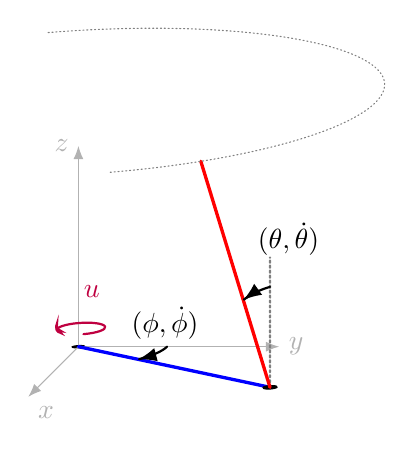
\begin{tikzpicture}[
		scale=1.50,
		line cap=round, line join=round,
		>=Latex,
		  % --- Custom "3D-like" basis: z up, y right, x forward (diagonal) ---
		x={(-0.25cm,-0.25cm)},   % x points "forward"
		y={(1.00cm,0.00cm)},    % y points right
		z={(0.00cm,1.00cm)}     % z points up
		]
		
		% ---------- Parameters (adjust if desired) ----------
		\def\Larm{2.4}      % actuated arm length
		\def\Lpend{2.2}     % pendulum length
		\def\phiang{35}     % nonzero phi angle (deg)
		\def\thetang{-20}    % nonzero theta from upward vertical (deg)
		% Small radii for angle arcs
		\def\rphi{0.85}
		\def\radth{0.85}
		
		% ---------- Base / pivot ----------
		\coordinate (O) at (0,0,0);
		\fill (O) circle[radius=0.06];
		
		% ---------- Reference axes (subtle) ----------
		\draw[->,thin,gray!60] (O) -- (1.7,0,0) node[below right] {$x$};
		\draw[->,thin,gray!60] (O) -- (0,1.7,0) node[right] {$y$};
		\draw[->,thin,gray!60] (O) -- (0,0,1.7) node[left] {$z$};
		
		% ---------- Input torque u about vertical axis ----------
		\def\ru{0.2}
		\def\zval{0.2}
		%\draw[thick, purple, ->] plot[domain=20:330, samples=60]({\ru*cos(\x)}, {\ru*sin(\x)}, 0);
		\begin{scope}[shift={(0, 0, 0.2)}]
			\draw[
			purple, 
			thick, 
			-{Stealth[bend]}
			] (20:0.4) arc[start angle=20, end angle=330, radius=\ru];
		\end{scope}
		\node[purple] at ($(O)+(0.55,0.25,0.60)$) {$u$};
		
		% ---------- Actual arm (nonzero phi) ----------
		% Arm direction in x-y plane, measured from +y toward +x:
		% A = Larm * (sin(phi) in x, cos(phi) in y, 0 in z)
		\coordinate (A) at ({\Larm*sin(\phiang)},{\Larm*cos(\phiang)},{0});
		\draw[very thick, blue] (O) -- (A);
		
		% ---------- Show phi angle arc (from dotted ref to arm) ----------
		% Small arc in horizontal plane around O
		\def\rphi{0.75}
		\draw[thick, ->] plot[domain=0:\phiang, samples=50]
		({\rphi*sin(\x)},{\rphi*cos(\x)},0);
		%\draw[->,thick] ({\rphi*sin(\phiang)},{\rphi*cos(\phiang)},0) -- ++(0.001,0.001,0);
		\node at ({0.95*\rphi*sin(\phiang/2)},{1.10*\rphi*cos(\phiang/2)},0.25) {$(\phi, \dot{\phi})$};
		
		
		% ---------- Pendulum joint at arm end ----------
		\filldraw[black] (A) circle[radius=0.06];
		
		% ---------- Zero-reference for theta (dotted) ----------
		% Convention: theta=0 points upward along +z at joint A
		\coordinate (Rth) at ($(A)+(0,0,0.5*\Lpend)$);
		\draw[densely dotted,thick,gray] (A) -- (Rth);
		
		% ---------- Actual pendulum (nonzero theta) ----------
		% Furuta pendulum swings in a vertical plane orthogonal to arm:
		% unit arm direction e_arm = (sin phi, cos phi, 0)
		% unit perpendicular in x-y plane e_perp = (-cos phi, sin phi, 0)
		\pgfmathsetmacro{\ex}{-cos(\phiang)}
		\pgfmathsetmacro{\ey}{ sin(\phiang)}
		
		% Pendulum end point: P = A + Lpend*(sin(theta)*e_perp + cos(theta)*z)
		\coordinate (P) at ($ (A) + ({\Lpend*sin(\thetang)*\ex},{\Lpend*sin(\thetang)*\ey},{\Lpend*cos(\thetang)}) $);
		
		\draw[very thick, red] (A) -- (P);
		
		% ---------- Dotted circle through tip P in x-y plane ----------
		% Calculate the components of P in the XY-plane
		\pgfmathsetmacro{\Px}{\Larm*sin(\phiang) + \Lpend*sin(\thetang)*\ex}
		\pgfmathsetmacro{\Py}{\Larm*cos(\phiang) + \Lpend*sin(\thetang)*\ey}
		% Calculate radius with veclen
		\pgfmathsetmacro{\Rtip}{veclen(\Px,\Py)}
		% Height is z-coordinate of P
		\pgfmathsetmacro{\Pz}{\Lpend*cos(\thetang)}
		\draw[densely dotted, gray] plot[domain=20:200, samples=100] 
		({\Rtip*cos(\x)}, {\Rtip*sin(\x)}, \Pz);
		
		% ---------- Show theta angle arc (from dotted vertical to pendulum) ----------
		% theta arc in the plane spanned by z and e_perp (from +z to pendulum)
		\begin{scope}[shift={(A)}]
			\draw[thick, ->] plot[domain=0:\thetang, samples=50] 
			({\radth*sin(\x)*\ex}, {\radth*sin(\x)*\ey}, {\radth*cos(\x)});
		\end{scope}
		\node at ($ (A) + ({0.92*\radth*sin(\thetang/2)*\ex},{0.92*\radth*sin(\thetang/2)*\ey},{0.92*\radth*cos(\thetang/2)}) + (0.15,0.30,0.55)$) {$(\theta, \dot{\theta})$};
		
	\end{tikzpicture}
	\caption{Isometric schematic of the Furuta pendulum in a non-zero configuration. Dotted lines indicate the zero-angle references for $\phi$ (horizontal arm) and $\theta$. Curved arrows show the non-zero angles. The torque input $u$ acts about the $z$-axis (rotation in the $x$--$y$ plane).}
	\label{fig:furuta_tikz_iso}
\end{figure}

\subsection{Mechanical model}

The Furuta pendulum consists of a horizontally rotating actuated arm (angle $\phi$) with a passive pendulum attached (angle $\theta$) moving in a vertical plane. Notice that $\theta=0$ represents the upward unstable equilibrium. We use the state vector
\begin{equation}
	x := (\phi,\theta,\dot{\phi},\dot{\theta})^\top,
\end{equation}
and a partition
\begin{equation}
	x_1 := (\phi,\dot{\phi})^\top, \qquad x_2 := (\theta,\dot{\theta})^\top,
	\label{eq:furuta_partition}
\end{equation}
which reflects collocated sensing/actuation on the actuated joint and partial observability of the passive joint. We adopt Gäfvert’s Furuta-pendulum model, which provides an Euler-Lagrange description $$M(q)\ddot q + C(q,\dot q)\dot q + g(q) + \tau_f(q,\dot q)=\tau,$$ with underactuation $\tau=(u,0)^\top$ with closed-form expressions for inertia $M(q)$,  coriolis/centripetal matrix $C(q,\dot q)$ and gravity force vector $g(q)$ and physically identified parameter values \citep{Gafvert1998}. .

To make the passive dynamics genuinely uncertain in a configuration-dependent way, we introduce a directional viscous friction model on the passive joint:
\begin{equation}
	\tau_{f,\theta}(\theta,\dot{\theta}) = b_\theta(\theta)\dot{\theta},
	\label{eq:dir_friction}
\end{equation}
with
\begin{equation}
	b_\theta(\theta) = b_0 + b_1\cos^2\theta, \quad b_0,b_1>0.
\end{equation}
This choice is intentionally simple yet structured: it induces a varying mean friction level across the configuration manifold, which can degrade prediction if the estimator assumes an incorrect friction profile.
Furthermore, the measurements are collocated on the actuated joint:
\begin{equation}
	y_k = \phi(t_k) + v_k, \qquad v_k\sim\mathcal{N}(0,\sigma_\phi^2),
	\label{eq:furuta_meas}
\end{equation}
corresponding to a partial, noisy observation of the full state.

The proposed model is a standard mechanical system and can be embedded into \eqref{eq:pH} by using energy variables. Concretely, define
\begin{equation}
	x = (q,p) \in \mathbb{R}^{4},\qquad p := M(q)\dot q,
	\label{eq:furuta_energy_state}
\end{equation}
and choose a Hamiltonian $H(q,p)=\tfrac12 p^\top M^{-1}(q)p + V(q)$ where $\nabla V(q)=g(q)$.
The dissipation matrix $R(x)$ in \eqref{eq:pH} is chosen so that its dissipative contribution reproduces $\tau_f(q,\dot q)$ in \eqref{eq:dir_friction}, while the skew interconnection $J(x)$ contains the canonical mechanical interconnection together with the (power-preserving) velocity-coupling structure represented by $C(q,\dot q)\dot q$. The input matrix $B$ and measurement map $h(\cdot)$ are set to reflect underactuation ($\tau=(u,0)^\top$) and collocated sensing \eqref{eq:furuta_meas}.
Finally, structured modelling error in $b_\theta(\theta)$ is represented as an augmented-state random-walk parameter process, using a Fourier basis, with additive diffusion in the augmented coordinates. This yields an augmented stochastic pH instance of \eqref{eq:pH} on $\tilde x=(x^\top,c^\top)^\top$ with additive diffusion (constant $B$ in the augmented coordinates), so the case study remains within the modelling class assumed in Sections \ref{sec:notation} and \ref{sec:entropy}.

In the \emph{estimator}, we do not assume knowledge of the specific $\cos^2\theta$ form. Instead, we estimate an unknown, smooth periodic friction profile using a low-order Fourier basis of order 2:
\begin{equation}
	\hat{b}_\theta(\theta;\,c) = c_0 + c_1\cos\theta + s_1\sin\theta + c_2\cos(2\theta) + s_2\sin(2\theta),
	\label{eq:fourier_friction}
\end{equation}
where $c := (c_0,c_1,s_1,c_2,s_2)^\top$ are treated as additional (slowly varying) states with random-walk dynamics. This yields an augmented state $\tilde{x}:=(x^\top,c^\top)^\top$ and places the case study within the general stochastic framework via state augmentation: the augmented process noise captures slow parameter drift and unmodelled effects in a standard Kalman-type manner. In the simulations we enforce positivity of $\hat b_\theta(\theta;c)$ to avoid nonphysical negative damping while retaining differentiability for finite-difference Jacobians.

The benchmark is designed to isolate informational effects from controller design. We therefore use an exogenous probing torque $u(t)$ (multisine with frequency content $[0.2, 0.35, 0.6, 0.9]$ Hz and random phase shifts) applied to the actuated joint and keep the sensing modality fixed. 

To highlight estimator readiness rather than trivial rapid correction, we adopt a multirate filtering protocol: the plant is integrated at a fast step $\Delta t$, while the measurement update of the EKF is performed only every $\Delta t_{\mathrm{upd}}\gg \Delta t$ (e.g.\ $40$\,ms), with prediction steps in between. This regime is representative of practical constraints where control/simulation may run faster than estimation or parameter adaptation, and it makes multi-step prediction and parameter learning sensitive to how effectively information about $x_2$ is routed into the measured channel.

The goal is to introduce an additional skew-symmetric coupling matrix to \eqref{eq:pH} of the form \eqref{eq:Jtheta} to improve information routing. But first $kappa_i=0$ is studied to establish a baseline case. We evaluate the information metrics from Section~\ref{sec:info-metrics} on this baseline to identify configuration-dependent bottlenecks before introducing skew interconnection shaping.

\subsection{Baseline case: no gyroscopic intervention}


% =========================================================
\section{Discussion}\label{sec:discussion}
The reversible flow induced by \(J(x)\) is measure--preserving. Nevertheless, \emph{how} the flow threads the state partition affects \emph{projected} uncertainty and predictability. In integrable limits, motion occurs on invariant tori; resonant frequency ratios yield structured (Lissajous--like) projections while incommensurate ratios produce dense coverage. With small noise and partial sensing, these geometric features map into peaks/dips of block MI and vector TE on the innovations. For interpretation (not for proofs), we refer to \emph{Resonant Information Manifolds (RIMs)}---regions where integer relations in local frequencies are approximately satisfied; they organize where information routing is most/least effective over short transients. A KAM--aware paragraph will be added in the case studies to discuss persistence of quasi--periodic structure under weak nonlinearity and small perturbations.


Our Furuta case study explicitly probes a multirate regime in which estimator updates are sparse relative to plant integration/control updates; in such regimes, multi-step prediction and parameter learning depend critically on how effectively information is routed into measured channels. This aligns with information-engine analyses where measurement noise and inference quality strongly constrain performance \cite{duBuisson2024_APX}.

% =========================================================
\section{Conclusion}
We established a nonlinear, Liouville--consistent framework in which the skew interconnection acts as an \emph{information router}: it cannot change total phase--volume or global belief entropy, but it can increase \emph{directional} predictability across a partition. With small noise and partial sensing, this routing is quantitatively captured by block MI and vector TE on innovations, and it has a provable estimator--level benefit: earlier time--to--certainty under fixed dissipation and diffusion. A low--dimensional parametric family \(J_\theta(x)\) enables geometric information control consistent with pH structure. Experiments will illustrate compact, credible gains on standard benchmarks.

% =========================================================
\bibliographystyle{elsarticle-num}
\bibliography{ref}

\end{document}